\documentclass[20pt,margin=1in,innermargin=-4.5in,blockverticalspace=-0.25in]{tikzposter}
\geometry{paperwidth=42in,paperheight=32.5in}
\usepackage[utf8]{inputenc}
\usepackage{amsmath}
\usepackage{amsfonts}
\usepackage{amsthm}
\usepackage{amssymb}
\usepackage{mathrsfs}
\usepackage{graphicx}
\usepackage{adjustbox}
\usepackage{enumitem}
\usepackage[backend=biber,style=numeric]{biblatex}
\usepackage{uomtheme}

\usepackage{mwe} % for placeholder images

\addbibresource{refs.bib}

% set theme parameters
\tikzposterlatexaffectionproofoff
\usetheme{UoMTheme}
\usecolorstyle{UoMStyle}

\usepackage[scaled]{helvet}
\renewcommand\familydefault{\sfdefault} 
\usepackage[T1]{fontenc}


\title{Connectivity Matrix and its Application in Airline Flights}
\institute{Faculty of Computing and Information Technology}
\titlegraphic{
\includegraphics[width=0.06\textwidth]{pucit.png}}

% begin document
\begin{document}
\maketitle
\centering
\begin{columns}
    \column{0.32}
    \block{Introduction}{
     \vspace{1em}
        The purpose of this poster is to show how power of a matrix may be used to investigate graphs. Special attention is paid to airline route maps as example of graphs.\\
        An air transportation network consists of distinct airports (cities) and direct flight routes between airport pairs. 
        Usually a graph G(V,E) is used to describe an air transportation network, where the node set V represents all the n airports and the edge (link) set represent all the m direct flight routes between airports. Mostly if a direct flight route from airport 1 to airport 2 exists, the direct return route from airport 2 to airport 1 also exists. 
     \vspace{1em}
    }
    \block{Key Terms}{
    
    1.A graph is a set of points (called vertices, or nodes) and a set of lines called edges connecting some pairs of vertices.\\
    2. Two vertices connected by an edge are said to be adjacent.\\   
    3. Notice that two vertices may be connected by more than one edge (A and B are connected by 2 distinct edges), that a vertex need not be connected to any other vertex(D), and that a vertex may be connected to itself(F).\\
   \vspace{1em}
   \begin{tikzfigure}
   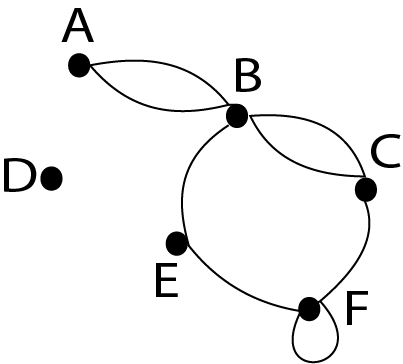
\includegraphics[width=0.08\textwidth]{graph.png}
    \end{tikzfigure}

     \vspace{1em}
    4. According to various authors, we can distinguish between two basic perspectives on connectivity:\\
    (1) the accessibility 
    perspective or (in)direct connectivity\\ 
    (2) the centrality or hub connectivity perspective.\\
   Whereas the first perspective considers the number and quality of direct and indirect air travel connections available to the consumer at a certain airport, the second perspective measures 
   the number of transfer opportunities available via a specific airport.
     \vspace{1em}
       }
    \block{Proposed Methodology}{
     \vspace{1em}
        Let's consider some airlines some from Pakistan to different Europe countries e.g. Spain, Italy, Norway, France and Denmark while Dubai is serving as a HUB for all these countries.\\
        The various routes among the countries are represented in the graph.\\
        Several questions arise, How many routes from country A to country B require exactly three connectivity flights?How many routes require no more than four flights-and so forth?Since this particular network is small, these questions can be answered by "eyeballing" the diagram. But the eye-ball method won't get you very far with the large networks which occur in a more practical situation. Let's see how matrix algebra can be applied.\\ 
        Begin by creating a connectivity matric C = [ $c_{ij}$ ] (also known as an adjacency matrix) in which\\ 
        \vspace{1em}
        $c_{ij}$ = 0 - if there is no flight from city i to city j\\
        $c_{ij}$ = 1 - if there is a flight from city i to city j
        \vspace{1em}
    }

    \column{0.36}
    \block{Mathematical Calculation}{
     Let's begin with supposing an airline network of Emirates\\
    \vspace{1em}
    \begin{tikzfigure}
    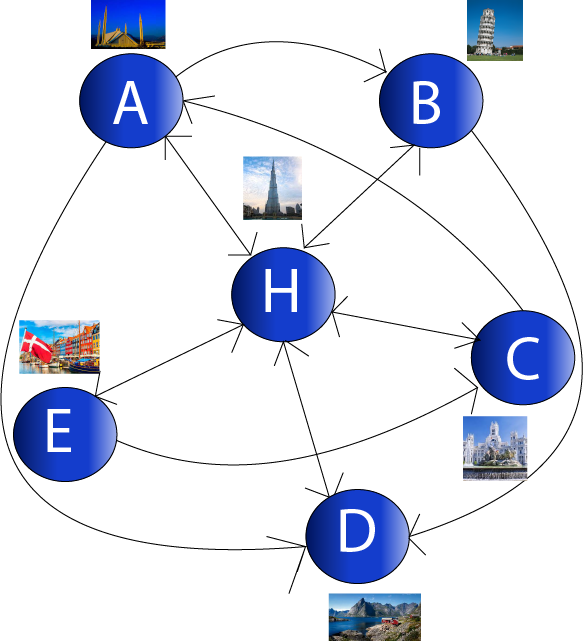
\includegraphics[width=0.21\textwidth]{lakaproj.png}
    \end{tikzfigure}
     \vspace{1em}
     Let, A: Islamabad, Pakistan\\
          B: Milan, Italy\\ 
          C: Madrid, Spain\\
          D: Oslo, Norway\\
          E: Paris, France\\
          H: Dubai, UAE\\
    The connectivity matrix of the above graph will be\\

    \begin{center}

        C = 
    \begin{pmatrix}
    
            - & A & B & C & D & E & F\\
      A &   0 & 1 & 0 & 1 & 0 & 1\\
      B &   0 & 0 & 0 & 1 & 0 & 1\\  
      C &   1 & 0 & 0 & 0 & 0 & 1\\
      D &   0 & 0 & 0 & 0 & 0 & 1\\
      E &   0 & 0 & 1 & 0 & 0 & 1\\
      H &   1 & 1 & 1 & 1 & 1 & 0\\
    \end{pmatrix}
    \end{center}
    \vspace{1em}
        The matrix C together with its powers $C^2, C^3, C^4,.....$ will provide all of the information needed to analyze the network, notice that since $c_{ik}$ is the number of direct routes from city i to city k, and since $c_{kj}$ is the number of direct routes from
        city k to city j, it follows that $c_{ik}c_{kj}$ must be the number of 2 flight routes from city i to city j that have a connection at 
        city k.\\ Consequently the (i,j) entry in the product $C^2$ = CC is\\
        $[C^2]_{ij} =  \sum_{k=1}^{5} c_{ik}c_{kj}$ = the total number of 2-route flights from city i to city j.\\
        Similarly, the (i,j)-entry in the product $C^3$ = CCC is\\
        $[C^3]_{ij} =  \sum_{k_{1},k_{2}=1}^{5}$ \space\space\space\space\space\space\space\space\space\space\space\space\space\space\space $c_{ik_{1}}c_{k_{1}k_{2}}c_{k_{2}j}$ = the total number of 3-route flights from city i to city j,and, in general,\\
        $[C^n]_{ij} =  \sum_{k_{1},k_{2}...k_{n-1}=1}^{5}$\space\space\space\space\space\space\space\space\space $c_{ik_{1}}c_{k_{1}k_{2}}....c_{k_{n-2}k_{n-1}c_{k_{n-1}j}}$
        
    }

    \column{0.32}
    \block{Results}{
         For our particular network,\\
         $C^2$ =
         \begin{pmatrix}
         1 & 1 & 1 & 2 & 1 & 2\\
         1 & 1 & 1 & 1 & 1 & 1\\
         1 & 2 & 1 & 2 & 1 & 1\\
         1 & 1 & 1 & 1 & 1 & 0\\
         2 & 1 & 1 & 1 & 1 & 1\\
         1 & 1 & 1 & 2 & 0 & 5
         \vspace{1em}
         \end{pmatrix}
         ,$C^3$ = 
        \begin{pmatrix}
         3 & 3 & 3 & 4 & 2 & 6\\
         2 & 2 & 2 & 3 & 1 & 5\\
         2 & 2 & 2 & 4 & 1 & 7\\
         1 & 1 & 1 & 2 & 0 & 5\\
         2 & 3 & 2 & 4 & 1 & 6\\
         6 & 6 & 5 & 7 & 5 & 5
         \vspace{1em}
         \end{pmatrix}
        ,$C^4$ = 
        \begin{pmatrix}
         9 & 9 & 8 & 12 & 6 & 15\\
         7 & 7 & 6 & 9 & 5 & 10\\
         9 & 9 & 8 & 11 & 7 & 11\\
         6 & 6 & 5 & 7 & 5 & 5\\
         8 & 8 & 7 & 11 & 6 & 12\\
         10 & 11 & 10 & 17 & 5 & 29\\
         \vspace{1em}
         \end{pmatrix}\\
         \vspace{1em}
         and\\
         $C$ + $C^2$ + $C^3$ + $C^4$ =
        \begin{pmatrix}
         13 & 14 & 12 & 19 & 9 & 12\\
         10 & 10 & 9 & 14 & 7 & 17\\
         13 & 13 & 11 & 17 & 9 & 20\\
         8 & 8 & 7 & 10 & 6 & 11\\
         12 & 12 & 11 & 16 & 8 & 20\\
         18 & 19 & 17 & 27 & 11 & 39
         \vspace{1em}
         \end{pmatrix}\\
        \vspace{1em}
        \vspace{1em}\\
         The fact that $[C^3]_{12}$ = 2 means there are exactly 2 three-flight routes from country A to country B, and $[C^4]_{12}$ = 5 means there is exactly 5 four-flight route-try to identify them. Furthermore, |$C$ + $C^2$ + $C^3$ + $C^4$| = 13 means that there are 13 routes from city A to city B that require no more than four flights.
        \vspace{1em}\\
         However, this assumption may not hold true on a more complex network because of a larger
            number of indirect paths which are not considered in the connectivity matrix. For example, when
            connecting hundreds of flights to fit schedules, liking cities together, and other factors requires a
            further complex network that involves deeper analysis. That sort of job is left to the
            professionals. For our particular network, we examined one of the most basic forms of
            connectivity matrix and its application to airline flights.
    }
    \block{References}{
        \vspace{-1em}
        \vspace{1em}\\
        1. http://www.math.utah.edu/~gustafso/s2019/2270/labs/lab3-adjacency.pdf\\
        2. https://www.researchgate.net/publicationCoverPdf\\
        3. https://cpb-us-w2.wpmucdn.com\\
        4. https://www.emirates.com/pk
        
    \vspace{1em}
    \begin{tikzfigure}
    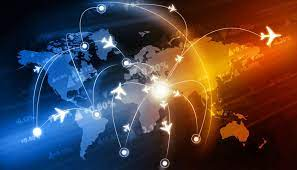
\includegraphics[width=0.25\textwidth]{final.jpg}
    \end{tikzfigure}
    }
    \block{Team Members}{
    Rida Shabbir (bcsf20m541)\\ Rida Fatima  (bcsf20m509)
        \begin{footnotesize}
        \printbibliography[heading=none]
        \end{footnotesize}
    }
\end{columns}
\end{document}